\begin{questions}
\question{
  Sketchs
}

\begin{solution}

By definition, the qubic harmonics for $d$ states are the following.
\begin{eqnarray}
  d_{3z^2-1} = Y_{2,0} = \sqrt{\frac{5}{16\pi}}\left( 3\cos^2\theta -1\right) \label{qub:1}\qquad\\
  d_{zx} = \sqrt{\frac{1}{2}} \left(Y_{2,-1}- Y_{2,1} \right) = \sqrt{\frac{5}{16\pi}}\sin{2\theta}\cos{\phi}  \label{qub:2}\\
  d_{yz} = \sqrt{\frac{1}{2}} i\left(Y_{2,-1}+ Y_{2,1} \right) = \sqrt{\frac{5}{16\pi}}\sin{2\theta}\sin{\phi} \label{qub:3}\\
  d_{x^2-y^2} = \sqrt{\frac{1}{2}} \left(Y_{2,-2} +Y_{2,2} \right) = \sqrt{\frac{5}{16\pi}}\sin^2{\theta}\cos{2\phi} \label{qub:4}\\
  d_{xy} = \sqrt{\frac{1}{2}}i \left(Y_{2,-2}- Y_{2,2} \right) = \sqrt{\frac{5}{16\pi}}\sin^2{\theta}\sin{2\phi} \label{qub:5}
\end{eqnarray}

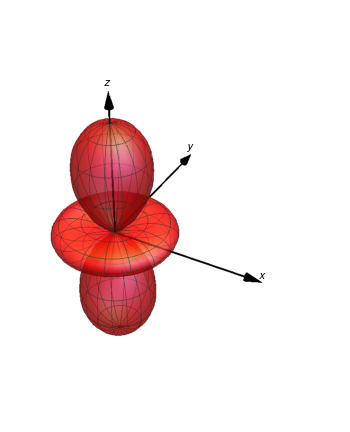
\includegraphics[width=50mm]{1.png}
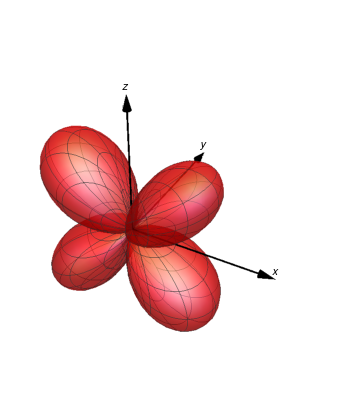
\includegraphics[width=50mm]{2.png}
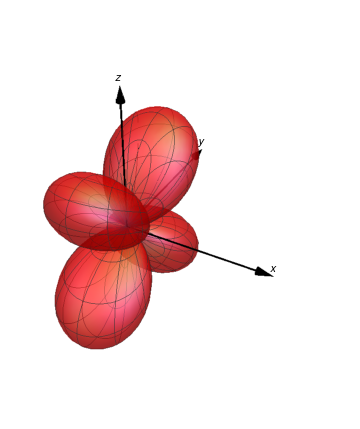
\includegraphics[width=50mm]{3.png}

\hspace{1.5cm}a)\hspace{5cm}b)\hspace{5cm}c)

\hspace{3cm}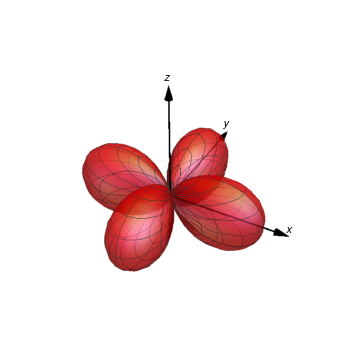
\includegraphics[width=50mm]{4.png}
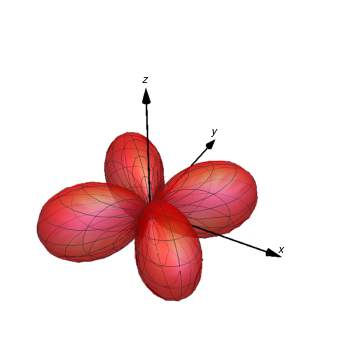
\includegraphics[width=50mm]{5.png}\label{5}

\hspace{5.2cm}d)\hspace{5cm}e)
 \captionof{figure}{Qubic harmonics, ploted as defined in eqs. \ref{qub:1}-\ref{qub:5}, and organized as follows a) $d_{3z^2-1}$, b) $d_{xz}$, c) $d_{yz}$, d) $d_{x^2-y^2}$, e) $d_{xy}$}

\end{solution}

\end{questions}
